% Created by tikzDevice version 0.12 on 2018-09-28 04:17:19
% !TEX encoding = UTF-8 Unicode
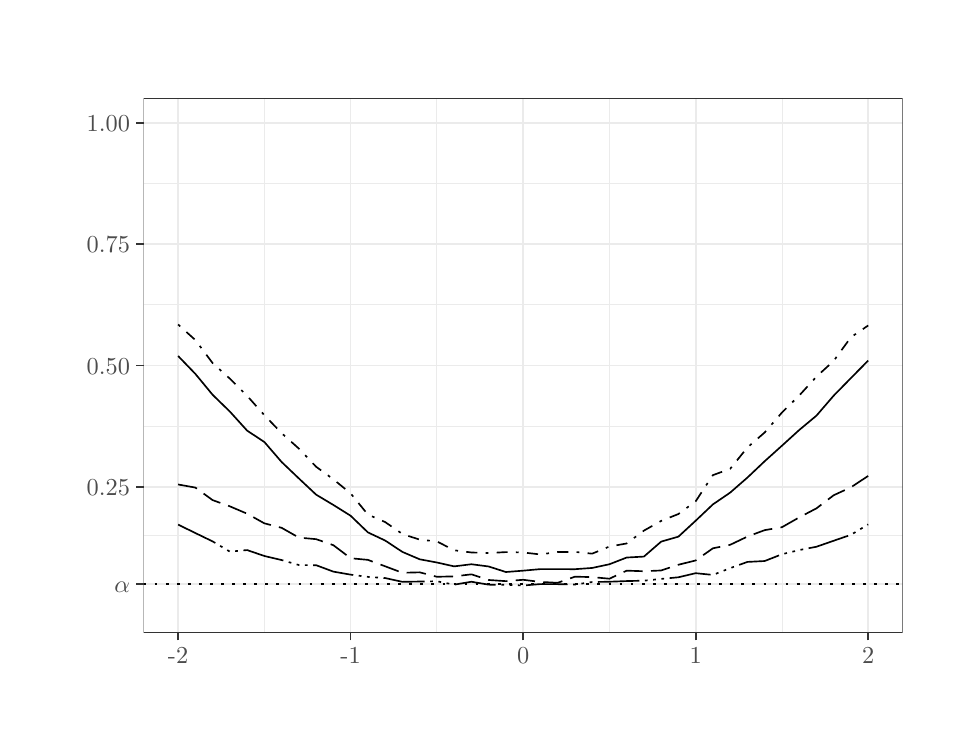
\begin{tikzpicture}[x=1pt,y=1pt]
\definecolor{fillColor}{RGB}{255,255,255}
\path[use as bounding box,fill=fillColor,fill opacity=0.00] (0,0) rectangle (325.21,252.94);
\begin{scope}
\path[clip] (  0.00,  0.00) rectangle (325.21,252.94);
\definecolor{drawColor}{RGB}{255,255,255}
\definecolor{fillColor}{RGB}{255,255,255}

\path[draw=drawColor,line width= 0.6pt,line join=round,line cap=round,fill=fillColor] (  0.00,  0.00) rectangle (325.21,252.94);
\end{scope}
\begin{scope}
\path[clip] ( 41.90, 34.26) rectangle (316.18,227.38);
\definecolor{fillColor}{RGB}{255,255,255}

\path[fill=fillColor] ( 41.90, 34.26) rectangle (316.18,227.38);
\definecolor{drawColor}{gray}{0.92}

\path[draw=drawColor,line width= 0.3pt,line join=round] ( 41.90, 69.37) --
	(316.18, 69.37);

\path[draw=drawColor,line width= 0.3pt,line join=round] ( 41.90,108.87) --
	(316.18,108.87);

\path[draw=drawColor,line width= 0.3pt,line join=round] ( 41.90,152.76) --
	(316.18,152.76);

\path[draw=drawColor,line width= 0.3pt,line join=round] ( 41.90,196.65) --
	(316.18,196.65);

\path[draw=drawColor,line width= 0.3pt,line join=round] ( 85.53, 34.26) --
	( 85.53,227.38);

\path[draw=drawColor,line width= 0.3pt,line join=round] (147.87, 34.26) --
	(147.87,227.38);

\path[draw=drawColor,line width= 0.3pt,line join=round] (210.21, 34.26) --
	(210.21,227.38);

\path[draw=drawColor,line width= 0.3pt,line join=round] (272.55, 34.26) --
	(272.55,227.38);

\path[draw=drawColor,line width= 0.6pt,line join=round] ( 41.90, 51.81) --
	(316.18, 51.81);

\path[draw=drawColor,line width= 0.6pt,line join=round] ( 41.90, 86.93) --
	(316.18, 86.93);

\path[draw=drawColor,line width= 0.6pt,line join=round] ( 41.90,130.82) --
	(316.18,130.82);

\path[draw=drawColor,line width= 0.6pt,line join=round] ( 41.90,174.71) --
	(316.18,174.71);

\path[draw=drawColor,line width= 0.6pt,line join=round] ( 41.90,218.60) --
	(316.18,218.60);

\path[draw=drawColor,line width= 0.6pt,line join=round] ( 54.37, 34.26) --
	( 54.37,227.38);

\path[draw=drawColor,line width= 0.6pt,line join=round] (116.70, 34.26) --
	(116.70,227.38);

\path[draw=drawColor,line width= 0.6pt,line join=round] (179.04, 34.26) --
	(179.04,227.38);

\path[draw=drawColor,line width= 0.6pt,line join=round] (241.38, 34.26) --
	(241.38,227.38);

\path[draw=drawColor,line width= 0.6pt,line join=round] (303.71, 34.26) --
	(303.71,227.38);
\definecolor{drawColor}{RGB}{0,0,0}

\path[draw=drawColor,line width= 0.6pt,dash pattern=on 1pt off 3pt on 4pt off 3pt ,line join=round] ( 54.37,145.67) --
	( 60.60,140.05) --
	( 66.83,131.73) --
	( 73.07,126.11) --
	( 79.30,119.90) --
	( 85.53,112.91) --
	( 91.77,106.41) --
	( 98.00,100.83) --
	(104.24, 94.27) --
	(110.47, 89.74) --
	(116.70, 84.64) --
	(122.94, 76.99) --
	(129.17, 74.29) --
	(135.40, 70.00) --
	(141.64, 67.93) --
	(147.87, 67.30) --
	(154.10, 64.10) --
	(160.34, 63.30) --
	(166.57, 63.09) --
	(172.81, 63.44) --
	(179.04, 63.30) --
	(185.27, 62.59) --
	(191.51, 63.47) --
	(197.74, 63.51) --
	(203.97, 62.87) --
	(210.21, 65.44) --
	(216.44, 66.56) --
	(222.68, 71.20) --
	(228.91, 74.71) --
	(235.14, 77.20) --
	(241.38, 81.80) --
	(247.61, 91.25) --
	(253.84, 93.53) --
	(260.08,101.25) --
	(266.31,106.66) --
	(272.55,113.86) --
	(278.78,120.00) --
	(285.01,126.81) --
	(291.25,132.54) --
	(297.48,141.07) --
	(303.71,145.32);

\path[draw=drawColor,line width= 0.6pt,dash pattern=on 15pt off 2pt on 1pt off 2pt on 1pt off 2pt on 1pt off 2pt ,line join=round] ( 54.37, 73.37) --
	( 60.60, 70.32) --
	( 66.83, 67.30) --
	( 73.07, 63.61) --
	( 79.30, 64.17) --
	( 85.53, 62.03) --
	( 91.77, 60.56) --
	( 98.00, 58.77) --
	(104.24, 58.70) --
	(110.47, 56.38) --
	(116.70, 55.29) --
	(122.94, 54.48) --
	(129.17, 54.06) --
	(135.40, 52.69) --
	(141.64, 52.80) --
	(147.87, 52.90) --
	(154.10, 51.67) --
	(160.34, 52.73) --
	(166.57, 51.67) --
	(172.81, 51.64) --
	(179.04, 51.36) --
	(185.27, 51.88) --
	(191.51, 51.85) --
	(197.74, 51.71) --
	(203.97, 52.62) --
	(210.21, 52.73) --
	(216.44, 52.97) --
	(222.68, 53.11) --
	(228.91, 53.75) --
	(235.14, 54.34) --
	(241.38, 55.82) --
	(247.61, 55.19) --
	(253.84, 57.64) --
	(260.08, 59.89) --
	(266.31, 60.21) --
	(272.55, 62.66) --
	(278.78, 64.17) --
	(285.01, 65.37) --
	(291.25, 67.54) --
	(297.48, 69.69) --
	(303.71, 73.44);

\path[draw=drawColor,line width= 0.6pt,dash pattern=on 7pt off 3pt ,line join=round] ( 54.37, 87.87) --
	( 60.60, 86.75) --
	( 66.83, 82.22) --
	( 73.07, 79.97) --
	( 79.30, 77.31) --
	( 85.53, 73.83) --
	( 91.77, 72.21) --
	( 98.00, 68.67) --
	(104.24, 68.11) --
	(110.47, 65.93) --
	(116.70, 61.22) --
	(122.94, 60.63) --
	(129.17, 58.31) --
	(135.40, 55.96) --
	(141.64, 56.13) --
	(147.87, 54.52) --
	(154.10, 54.66) --
	(160.34, 55.40) --
	(166.57, 53.36) --
	(172.81, 52.94) --
	(179.04, 53.43) --
	(185.27, 52.66) --
	(191.51, 52.34) --
	(197.74, 54.55) --
	(203.97, 54.41) --
	(210.21, 53.82) --
	(216.44, 56.73) --
	(222.68, 56.52) --
	(228.91, 56.80) --
	(235.14, 58.87) --
	(241.38, 60.42) --
	(247.61, 64.81) --
	(253.84, 66.07) --
	(260.08, 69.05) --
	(266.31, 71.37) --
	(272.55, 72.43) --
	(278.78, 75.97) --
	(285.01, 79.24) --
	(291.25, 83.98) --
	(297.48, 86.86) --
	(303.71, 90.96);

\path[draw=drawColor,line width= 0.6pt,line join=round] ( 54.37,134.29) --
	( 60.60,127.83) --
	( 66.83,120.28) --
	( 73.07,114.21) --
	( 79.30,107.33) --
	( 85.53,103.22) --
	( 91.77, 95.99) --
	( 98.00, 90.05) --
	(104.24, 84.19) --
	(110.47, 80.47) --
	(116.70, 76.57) --
	(122.94, 70.56) --
	(129.17, 67.62) --
	(135.40, 63.51) --
	(141.64, 60.84) --
	(147.87, 59.68) --
	(154.10, 58.28) --
	(160.34, 59.05) --
	(166.57, 58.24) --
	(172.81, 56.24) --
	(179.04, 56.73) --
	(185.27, 57.29) --
	(191.51, 57.29) --
	(197.74, 57.26) --
	(203.97, 57.71) --
	(210.21, 59.05) --
	(216.44, 61.47) --
	(222.68, 61.82) --
	(228.91, 67.23) --
	(235.14, 69.02) --
	(241.38, 74.78) --
	(247.61, 80.68) --
	(253.84, 84.93) --
	(260.08, 90.37) --
	(266.31, 96.27) --
	(272.55,101.88) --
	(278.78,107.54) --
	(285.01,112.73) --
	(291.25,119.97) --
	(297.48,126.32) --
	(303.71,132.64);

\path[draw=drawColor,line width= 0.6pt,dash pattern=on 1pt off 3pt ,line join=round] ( 41.90, 51.81) -- (316.18, 51.81);
\definecolor{drawColor}{gray}{0.20}

\path[draw=drawColor,line width= 0.6pt,line join=round,line cap=round] ( 41.90, 34.26) rectangle (316.18,227.38);
\end{scope}
\begin{scope}
\path[clip] (  0.00,  0.00) rectangle (325.21,252.94);
\definecolor{drawColor}{gray}{0.30}

\node[text=drawColor,anchor=base east,inner sep=0pt, outer sep=0pt, scale=  0.88] at ( 36.95, 48.78) {$\alpha$};

\node[text=drawColor,anchor=base east,inner sep=0pt, outer sep=0pt, scale=  0.88] at ( 36.95, 83.90) {$0.25$};

\node[text=drawColor,anchor=base east,inner sep=0pt, outer sep=0pt, scale=  0.88] at ( 36.95,127.79) {$0.50$};

\node[text=drawColor,anchor=base east,inner sep=0pt, outer sep=0pt, scale=  0.88] at ( 36.95,171.68) {$0.75$};

\node[text=drawColor,anchor=base east,inner sep=0pt, outer sep=0pt, scale=  0.88] at ( 36.95,215.57) {$1.00$};
\end{scope}
\begin{scope}
\path[clip] (  0.00,  0.00) rectangle (325.21,252.94);
\definecolor{drawColor}{gray}{0.20}

\path[draw=drawColor,line width= 0.6pt,line join=round] ( 39.15, 51.81) --
	( 41.90, 51.81);

\path[draw=drawColor,line width= 0.6pt,line join=round] ( 39.15, 86.93) --
	( 41.90, 86.93);

\path[draw=drawColor,line width= 0.6pt,line join=round] ( 39.15,130.82) --
	( 41.90,130.82);

\path[draw=drawColor,line width= 0.6pt,line join=round] ( 39.15,174.71) --
	( 41.90,174.71);

\path[draw=drawColor,line width= 0.6pt,line join=round] ( 39.15,218.60) --
	( 41.90,218.60);
\end{scope}
\begin{scope}
\path[clip] (  0.00,  0.00) rectangle (325.21,252.94);
\definecolor{drawColor}{gray}{0.20}

\path[draw=drawColor,line width= 0.6pt,line join=round] ( 54.37, 31.51) --
	( 54.37, 34.26);

\path[draw=drawColor,line width= 0.6pt,line join=round] (116.70, 31.51) --
	(116.70, 34.26);

\path[draw=drawColor,line width= 0.6pt,line join=round] (179.04, 31.51) --
	(179.04, 34.26);

\path[draw=drawColor,line width= 0.6pt,line join=round] (241.38, 31.51) --
	(241.38, 34.26);

\path[draw=drawColor,line width= 0.6pt,line join=round] (303.71, 31.51) --
	(303.71, 34.26);
\end{scope}
\begin{scope}
\path[clip] (  0.00,  0.00) rectangle (325.21,252.94);
\definecolor{drawColor}{gray}{0.30}

\node[text=drawColor,anchor=base,inner sep=0pt, outer sep=0pt, scale=  0.88] at ( 54.37, 23.25) {-2};

\node[text=drawColor,anchor=base,inner sep=0pt, outer sep=0pt, scale=  0.88] at (116.70, 23.25) {-1};

\node[text=drawColor,anchor=base,inner sep=0pt, outer sep=0pt, scale=  0.88] at (179.04, 23.25) {0};

\node[text=drawColor,anchor=base,inner sep=0pt, outer sep=0pt, scale=  0.88] at (241.38, 23.25) {1};

\node[text=drawColor,anchor=base,inner sep=0pt, outer sep=0pt, scale=  0.88] at (303.71, 23.25) {2};
\end{scope}
\end{tikzpicture}
